\chapter{Reconfigurations}

By the beginning of 1978, Ajahn Sumedho had departed Thailand and was
engaged in establishing a branch monastery in Britain. The tall American
ex-helicopter pilot who was skilled in crochet, Ajahn Pabakharo, had
been asked by Tan Ajahn Chah to take over leading the community at Wat
Pah Nanachat.

Around the beginning of 1978 a young, energetic, smiley English fellow
called Jeremy had arrived and was expressing interest in joining the
community. One morning, when he was diligently using a machete to chop
wood at the kitchen, he accidentally missed the piece of wood and
instead hacked into his foot. The reason I remember the incident is
because it fell to me to accompany him to see a doctor. In fact I ended
up physically carrying him into the local hospital. Jeremy was one of
those visitors who did settle in and make a commitment. He eventually
received \emph{upasampada} from Tan Ajahn Chah and the sangha at Wat Pah
Pong and was given the name Amaro Bhikkhu.

My carrying the not insignificant weight of Jeremy into hospital may or
may not have contributed to later that year myself entering hospital for
knee surgery. More likely it was down to the motorbike accident,
combined with hours of forcing myself to sit on the floor without a
cushion. I had gone to Bangkok to see if there was anything that could
be done about the increasing amount of pain I was having with my knees,
and the advice I received was that I needed a meniscectomy. In those
days that amounted to open surgery on both legs, and resulted in my
being in Ramathibodi hospital with both legs in full length plaster
casts for several weeks. Once the casts had been removed it became
apparent that the excessive growth of scar tissue had caused both knee
joints to seize up, requiring two more sessions of general anaesthetic
so the scar tissue could be torn. That was an ordeal I would not want to
have to repeat. Initially I had been told by the doctor that having both
knees done at the same time might mean being incapacitated for something
like three or four weeks. As it happened it was many weeks.

To my surprise, one day as I lay in bed in the hospital, I received a
visitor; it was ex-Tan Jotiko, now calling himself Mason Hamilton. When
Ajahn Sumedho had left for Britain the then Tan Jotiko had gone to live
at another, rather remote branch monastery called Wat Keurn. It wasn't
long, however, before he took the decision to renounce his commitment to
the robes and return to lay life. Of course, I was sad to see my friend
in this new form, but as far as I recall that it wasn't too big a deal.
Tan Varapañño had already disrobed by that time, so the perception
wasn't new, and finding myself stuck all alone in a Bangkok hospital for
weeks on end meant that I was already dealing with plenty of
disappointment; this was just a bit more.

Mason was staying with Geoff, an English friend and supporter of Wat Pah
Nanachat, and by the time I emerged from hospital the two of them had
organized a trip up to the north of Thailand, to Chiangmai. There we
would have the use of a quiet secluded house on the side of a forested
hill.

Before departing on that trip I had a chance to pay my respects to Tan
Ajahn Chah, who himself was in hospital in Bangkok. Seeing him again
meant a great deal. Having been for such a long time away from the
mother ship and its captain, it was encouraging to see Tan Ajahn Chah
once more. My knees were still not very flexible, so when I attempted to
get down on the floor to bow, I could hardly have been more awkward. I
started telling Tan Ajahn Chah, `It shouldn't be this way. The doctors
said it would only take a few weeks and here I am after all this time
and my knees are still not working properly.' He looked at me sternly,
and with an almost surprised expression at the degree of my foolishness
said, `What do you mean it shouldn't be this way? If it shouldn't be
this way it wouldn't be this way!' That was helpful. Thank you, Tan
Ajahn Chah. He wasn't implying anything like there being a big plan and
that the universe was teaching me a lesson; he was simply saying there
are causes and conditions for it to be this way, so stop resisting
reality. It \emph{is} like this! Such resistance only makes things
worse.

Mason, Geoff and I had a splendid road trip. The house on the side of
the hill, Doi Suthep, was Japanese-style and was surrounded by gorgeous
gardens and forest. Nearby was a waterfall that we could easily walk to.
During the day Geoff would sometimes drive us around to see some of the
sights, and at night it was quiet -- no more of the noise and fumes of
Bangkok traffic. That interlude was refreshing and renewing; thank you,
Geoff.

On one of those trips out, Geoff, Mason and I went as far as the next
province, Chiang Rai, where there was a small hermitage monastery
associated with Wat Pah Pong, called Wat Doi Dhamma Chedi. The abbot
there was Ajahn Koon, a short, young, enthusiastic and incredibly
talkative monk. Besides the welcome we received, there was a nearby
thermal hot pool where I was able to soak my still painful limbs. Ajahn
Koon generously invited me to stay there for the approaching Rains
Retreat (\emph{pansah}) and the thought of having access to the thermal
spring clinched it for me.

It was appropriate that I return to Wat Pah Nanachat to get permission
to be away for the Rains. By the time I reached there, there had been
another change in leadership. Now Ajahn Jagaro had been put in charge.
He was an Australian whose family were of Italian descent and he had a
big warm heart. He didn't hesitate to draw lines when they were needed,
but he did so with a warmth and sensitivity that commanded love and
respect from the community. There seemed to be no hesitation in giving
me permission to return to Chiang Rai province in the North.

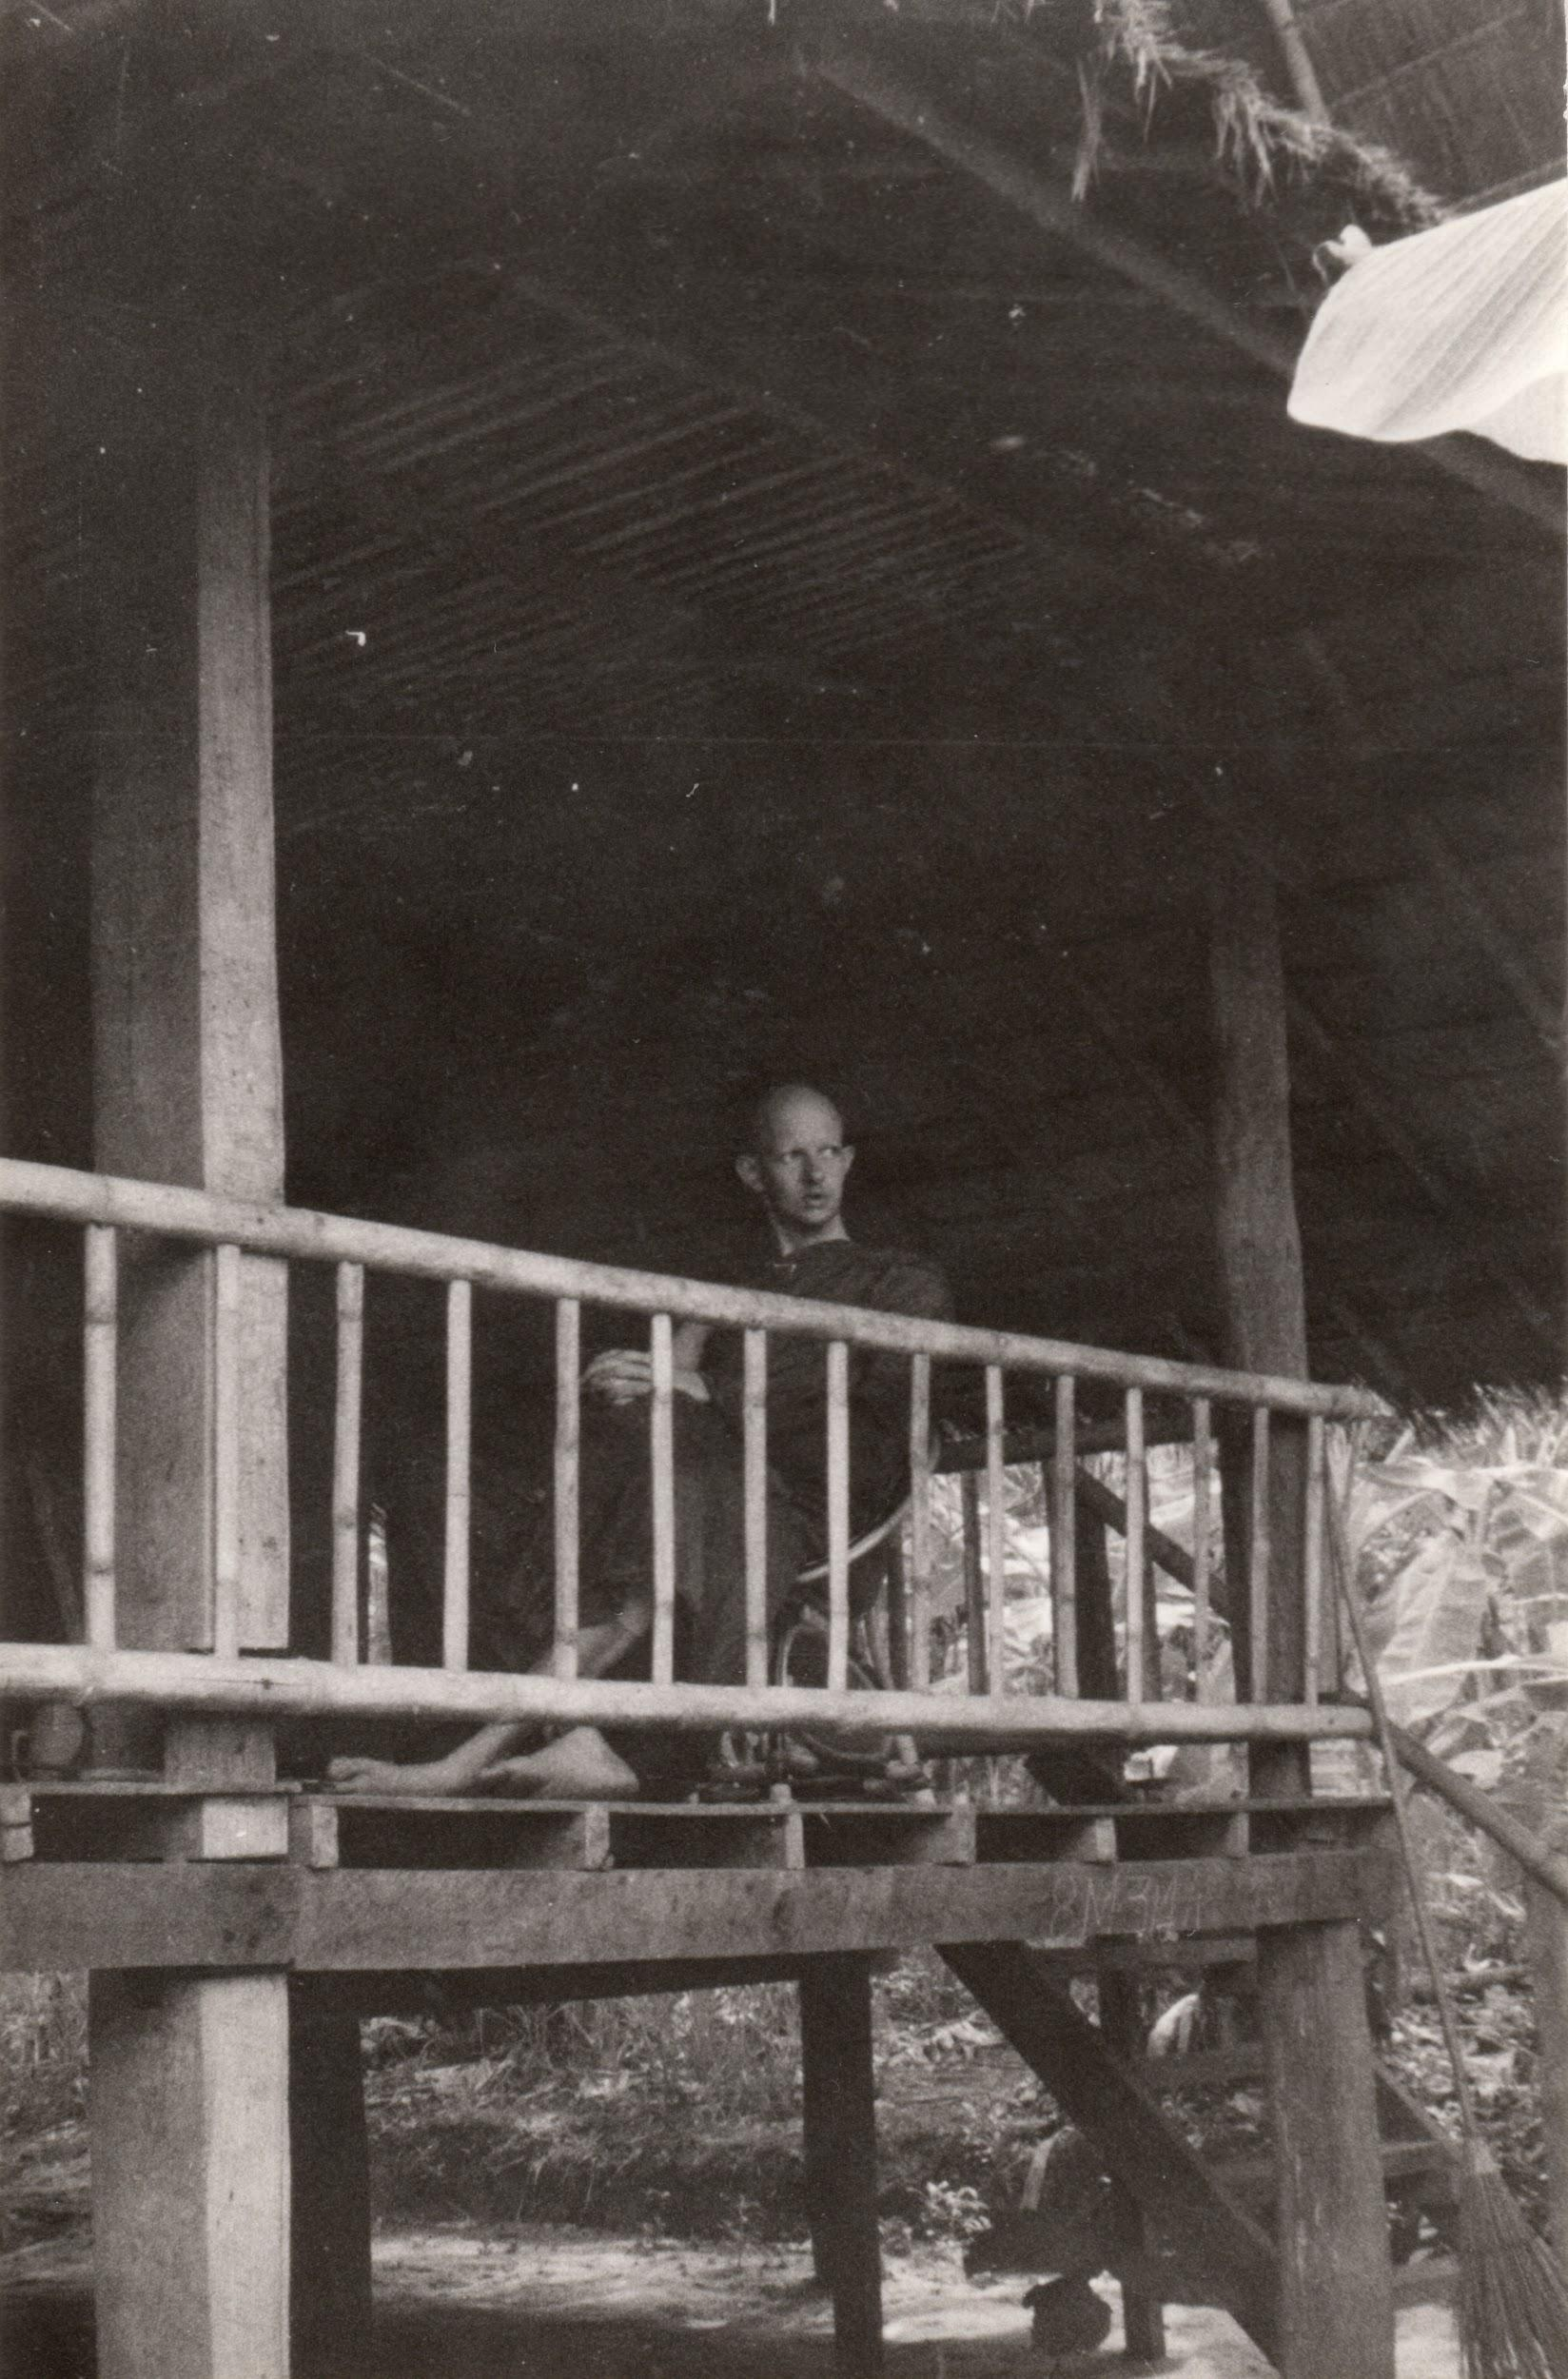
\includegraphics[width=2.14028in,height=3.23889in]{media/image3.jpeg}6
BURNING, BURNING, BURNING\\
~\\
Compared to Wat Pah Nanachat, at Wat Doi we were a relatively small
community of about seven monks and two novices. Nobody could speak
English, and that was a good fortune. I already had the basics of the
spoken language down, and now I was obliged to make use of it. During
this Rains Retreat something seemed to click, and I felt like I reached
a level of proficiency which made speaking with Thai people enjoyable,
not merely a struggle; I wasn't having to try so hard. Most days,
someone from the nearby village would drive me the two or three miles to
the thermal spring where, for perhaps an hour, I would soothe my legs.

During this period, the Canadian monk, Tan Tiradhammo, was living with
Tan Ajahn Chah at Wat Pah Pong. That year there were a large number of
junior monks in residence, and many of them were from Bangkok. This
meant that Tan Ajahn Chah regularly offered Dhamma talks spoken in the
Central Thai dialect. Most of the Western monks who had learnt to speak
Thai had learned that dialect; only a few were fluent in the Isaan
dialect. Tan Tiradhammo was thoughtfully sending me audio tapes by post,
and it was a delight to discover how well I could now understand them;
also I was motivated to start to work on translating at least one of
them into English. This was the talk now called, \emph{Reading The
Natural Mind}, and is printed in
\href{https://forestsangha.org/teachings/books/the-collected-teachings-of-ajahn-chah-single-volume?language=English}{\emph{\underline{The
Collected Teaching}} (Chapter 22, p 237) {[}41{]}.}

The exercise of translating proved particularly rewarding. It required
using my head to access conceptual meaning and word equivalents in both
languages, as well as the heart to sense the essential meaning that the
teacher was putting across. I vividly recall how in that \emph{Reading
The Natural Mind} talk, Tan Ajahn Chah was helpfully pointing out the
difference between the way wise beings and unwise beings relate to
wanting. Awakened beings relate to wanting with clear understanding so
they don't suffer. The rest of us still find identity by clinging to
wanting, and suffer accordingly. That opportunity was another gift.

Part way through that three-month retreat period, the monastery was
threatened with a forest fire. Fortunately Ajahn Koon had had the
foresight to create a firebreak around the vulnerable perimeter of the
monastery. After a lot of energetic sweeping the firebreak clear of
leaves, and skilful extinguishing of fires, the monastery was declared
safe again. Thinking about it later, firefighting struck me as a fitting
metaphor for the spiritual life. When we are on the front line dealing
with the flames, we can't be thinking too much about the bigger picture;
we can't know for sure the overall extent of the fire. However there are
those, our teachers and guides, who do have an overview; they can see
more than we can. It doesn't serve us well to be worrying about whether,
in terms of the bigger picture, we are succeeding in stopping the fire;
sometimes our task is to deal with the flames here and now, right in
front of us, and keep trusting.

It might have begun earlier, but from what I remember, this was the
first time that I registered another type of fire: an intense physical
sensation of burning. Sometimes my whole body felt like it was on fire,
at other times it was just my head. Where did all this heat come from?
Was it because of all the sugar I was consuming? There did seem to be a
correlation between taking a very sweet drink in the evening and shortly
afterwards having disturbingly strong symptoms of sweating and heart
racing. Or was it the kammic consequence of my misspent youth? If so, it
seemed a high price to pay for what, by comparison to others, was a
moderate amount of heedlessness. Maybe it was the result of how
unskilfully I approached meditation in the beginning, without an
appreciation for precepts and restraint. Or was this past life kamma?
Then again, if you trust in the theory of
\href{https://en.wikipedia.org/wiki/Epigenetics}{\underline{epigenetics}}
{[}42{]}, perhaps it was related to how my ancestors conducted
themselves?

I definitely didn't know what it was. It took a very long time -- and
here I mean years, not weeks or months -- to even begin to learn that
right practice meant training the whole body-mind to be able to simply
receive such sensations of being on fire, along with the not-knowing
state, and let it be. Trying to get rid of it, or to get over it -- and
often our attempts to understand are another sort of trying to get rid
of it -- only provides fuel which it feeds on.

It was during that period that one night I rolled over in my sleep and
landed on a scorpion. Understandably the scorpion stung me. I sat bolt
upright, putting my hand around to my back to find what had happened;
the critter must have taken that as another threat so it then stung my
hand. This was about 1 or 2 o'clock in the morning. I had received bites
from stinging ants before which were nasty, but this was my first
encounter with a scorpion. I was only guessing it was a scorpion as I
couldn't see anything. My heart was racing as was my mind: is there
anything I should do about it? The monastery I was in was a long way
away from any significant medical facility. Is there a chance I might
die? Should I be reciting \emph{Buddho, Buddho}? After some time the
pain subsided and I probably ended up going back to sleep. The next day,
back in my kuti after morning alms-round, I reached for a book that was
on a ledge above my bed and, just in time, I saw there was a scorpion
heading for my hand. I reacted quickly by throwing the book out the
window. I did feel bad about having possibly caused damage to the book;
but when I went outside and picked it up, I didn't feel terribly bad on
seeing it had landed in a way that meant the scorpion had been squashed.
My level of compassion was still not very well-developed.

